\subsection{Wichtige Berechnungen}
\label{sec:berechnungen}
Unter Anwendung der Formel für den schrägen Wurf, konnten die Geschwindigkeit und die notwendige Energie berechnet werden, 
die der Ball braucht um bis zum Korb zu fliegen. Die Berechnungen ergaben, dass die Bälle idealerweise in einer Höhe von ca. 40 cm und unter einem Winkel von ca. 50$^\circ$ abgeworfen werden. Für die Berechnungen wurde ein Rad mit ein Durchmesser von 15 cm benutzt.

\begin{figure}[h!]
	\begin{subfigure}{.5\textwidth}
		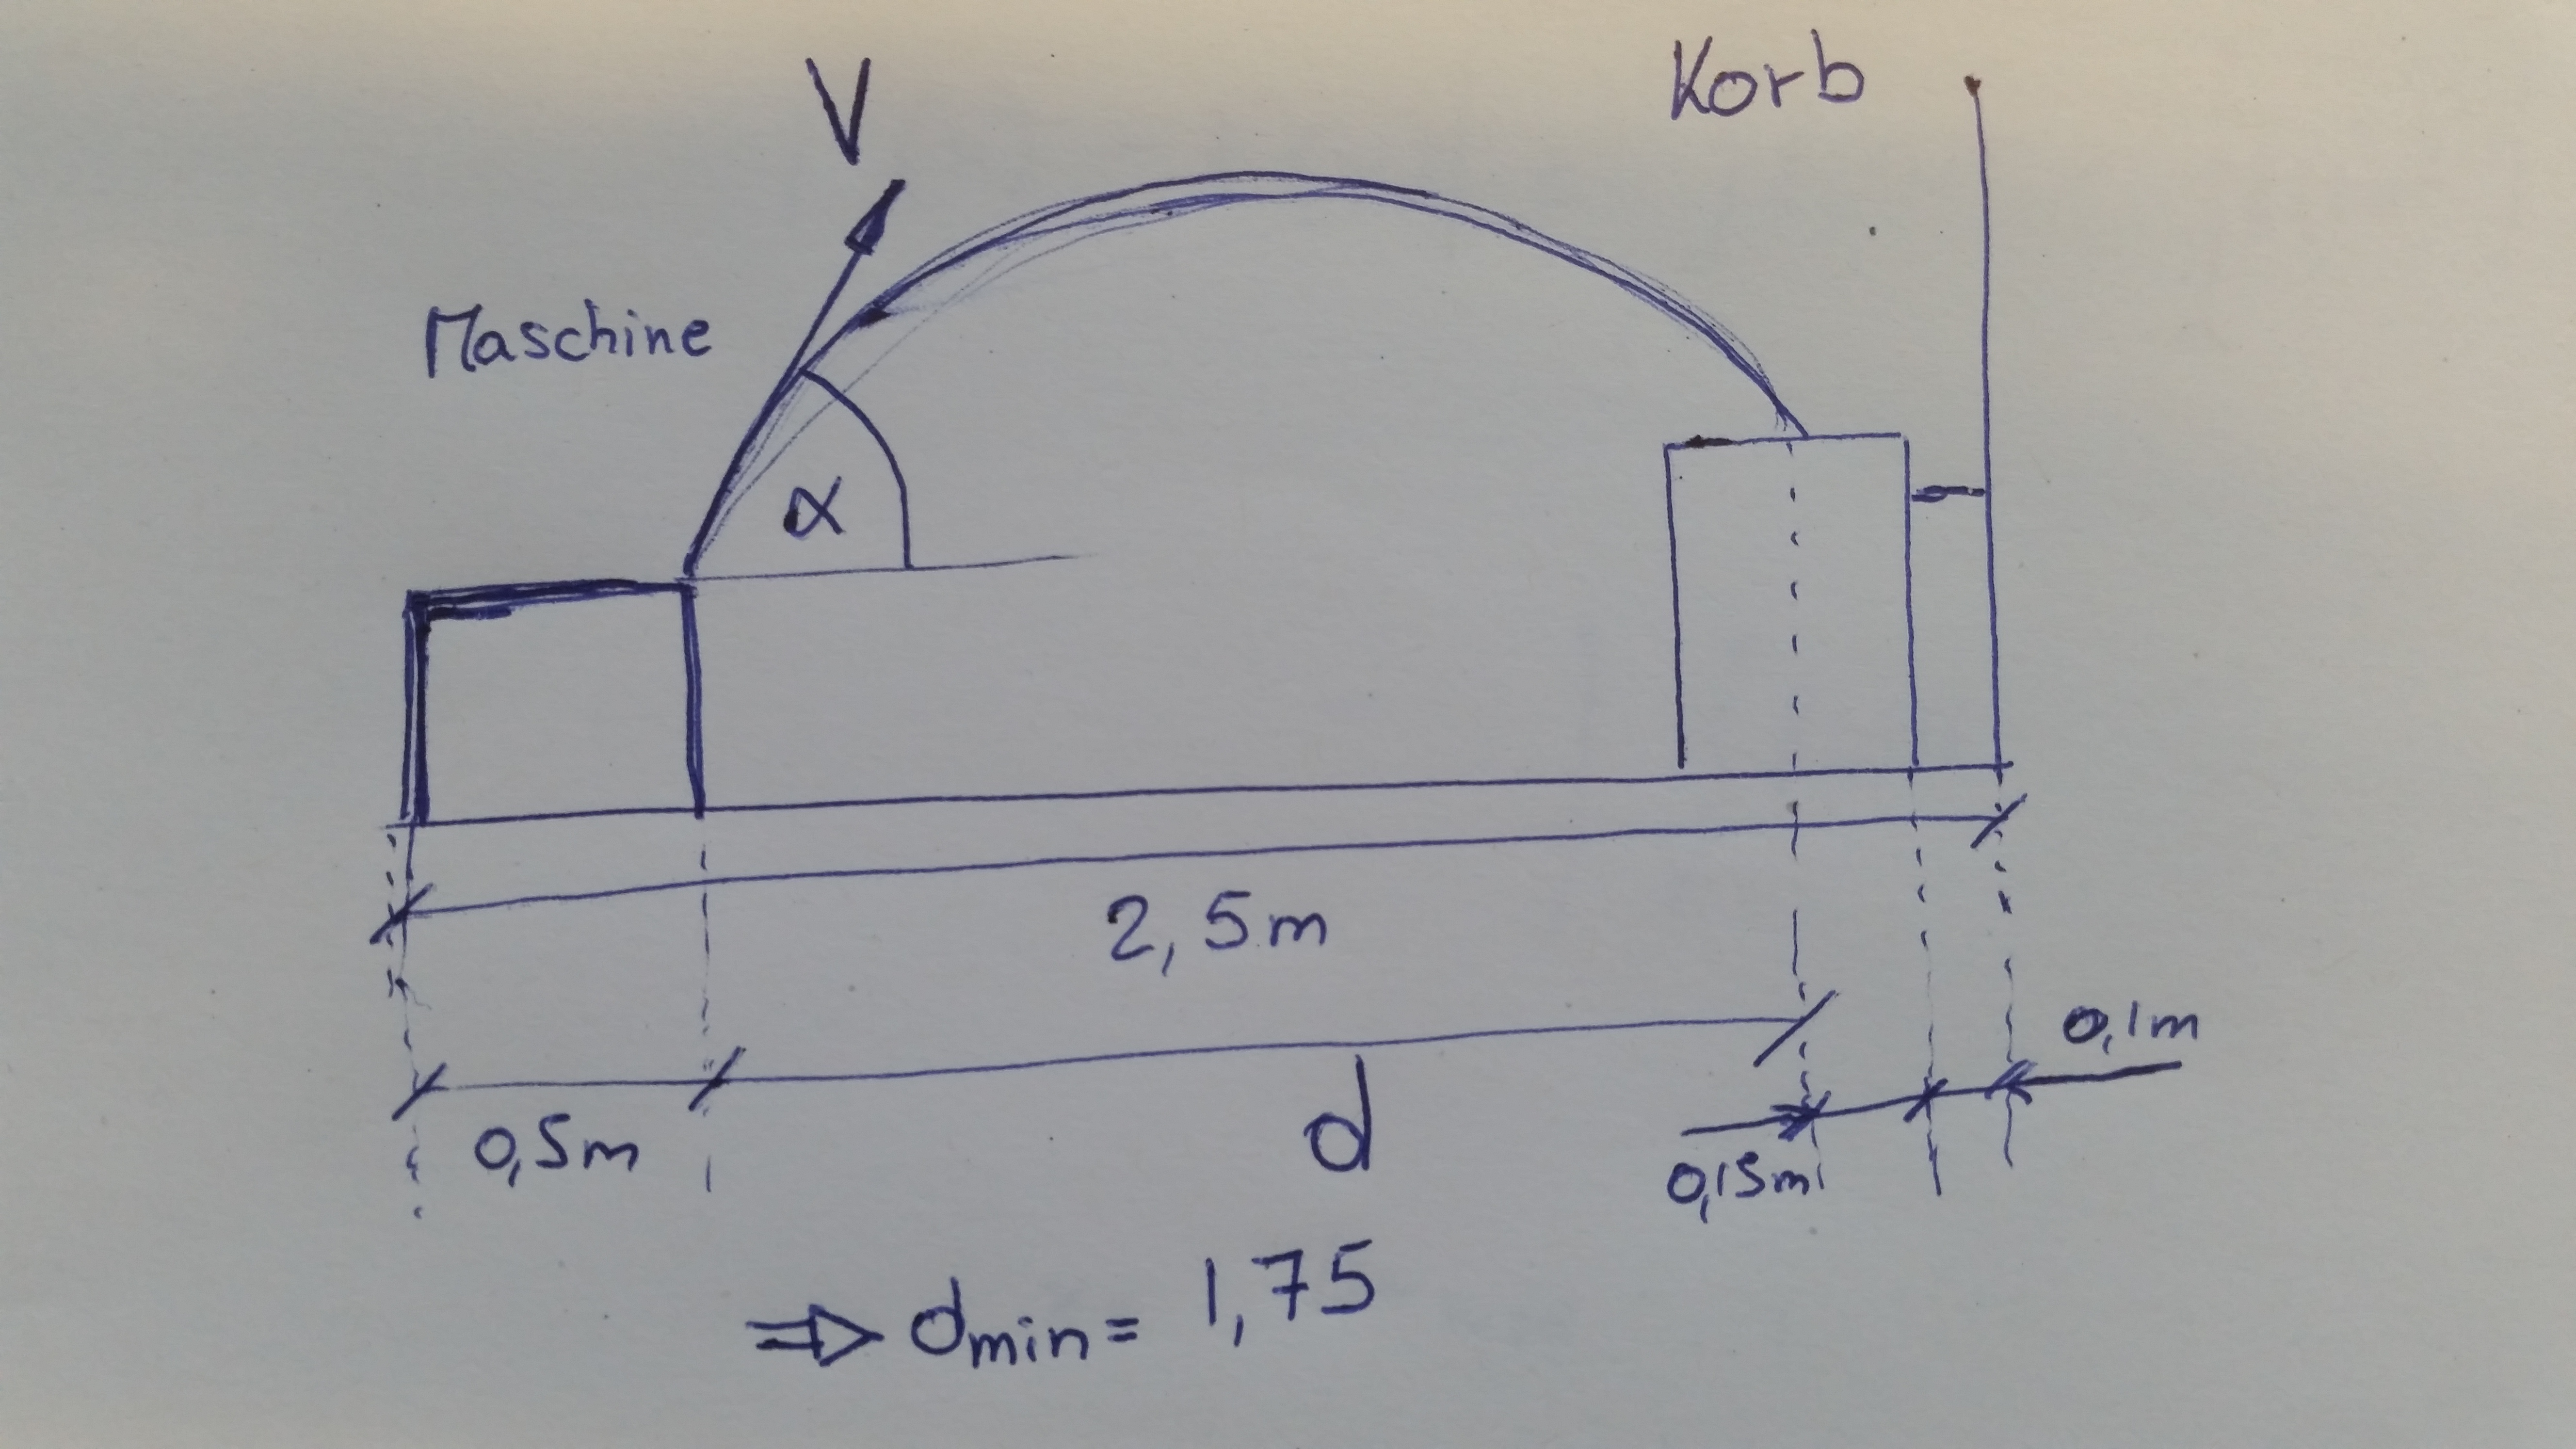
\includegraphics[width=1\textwidth]{../../fig/Skizze_Berechnung_1.jpg}
		\caption{Schräger Wurf von der Seite}
	\end{subfigure}
	\begin{subfigure}{.5\textwidth}
		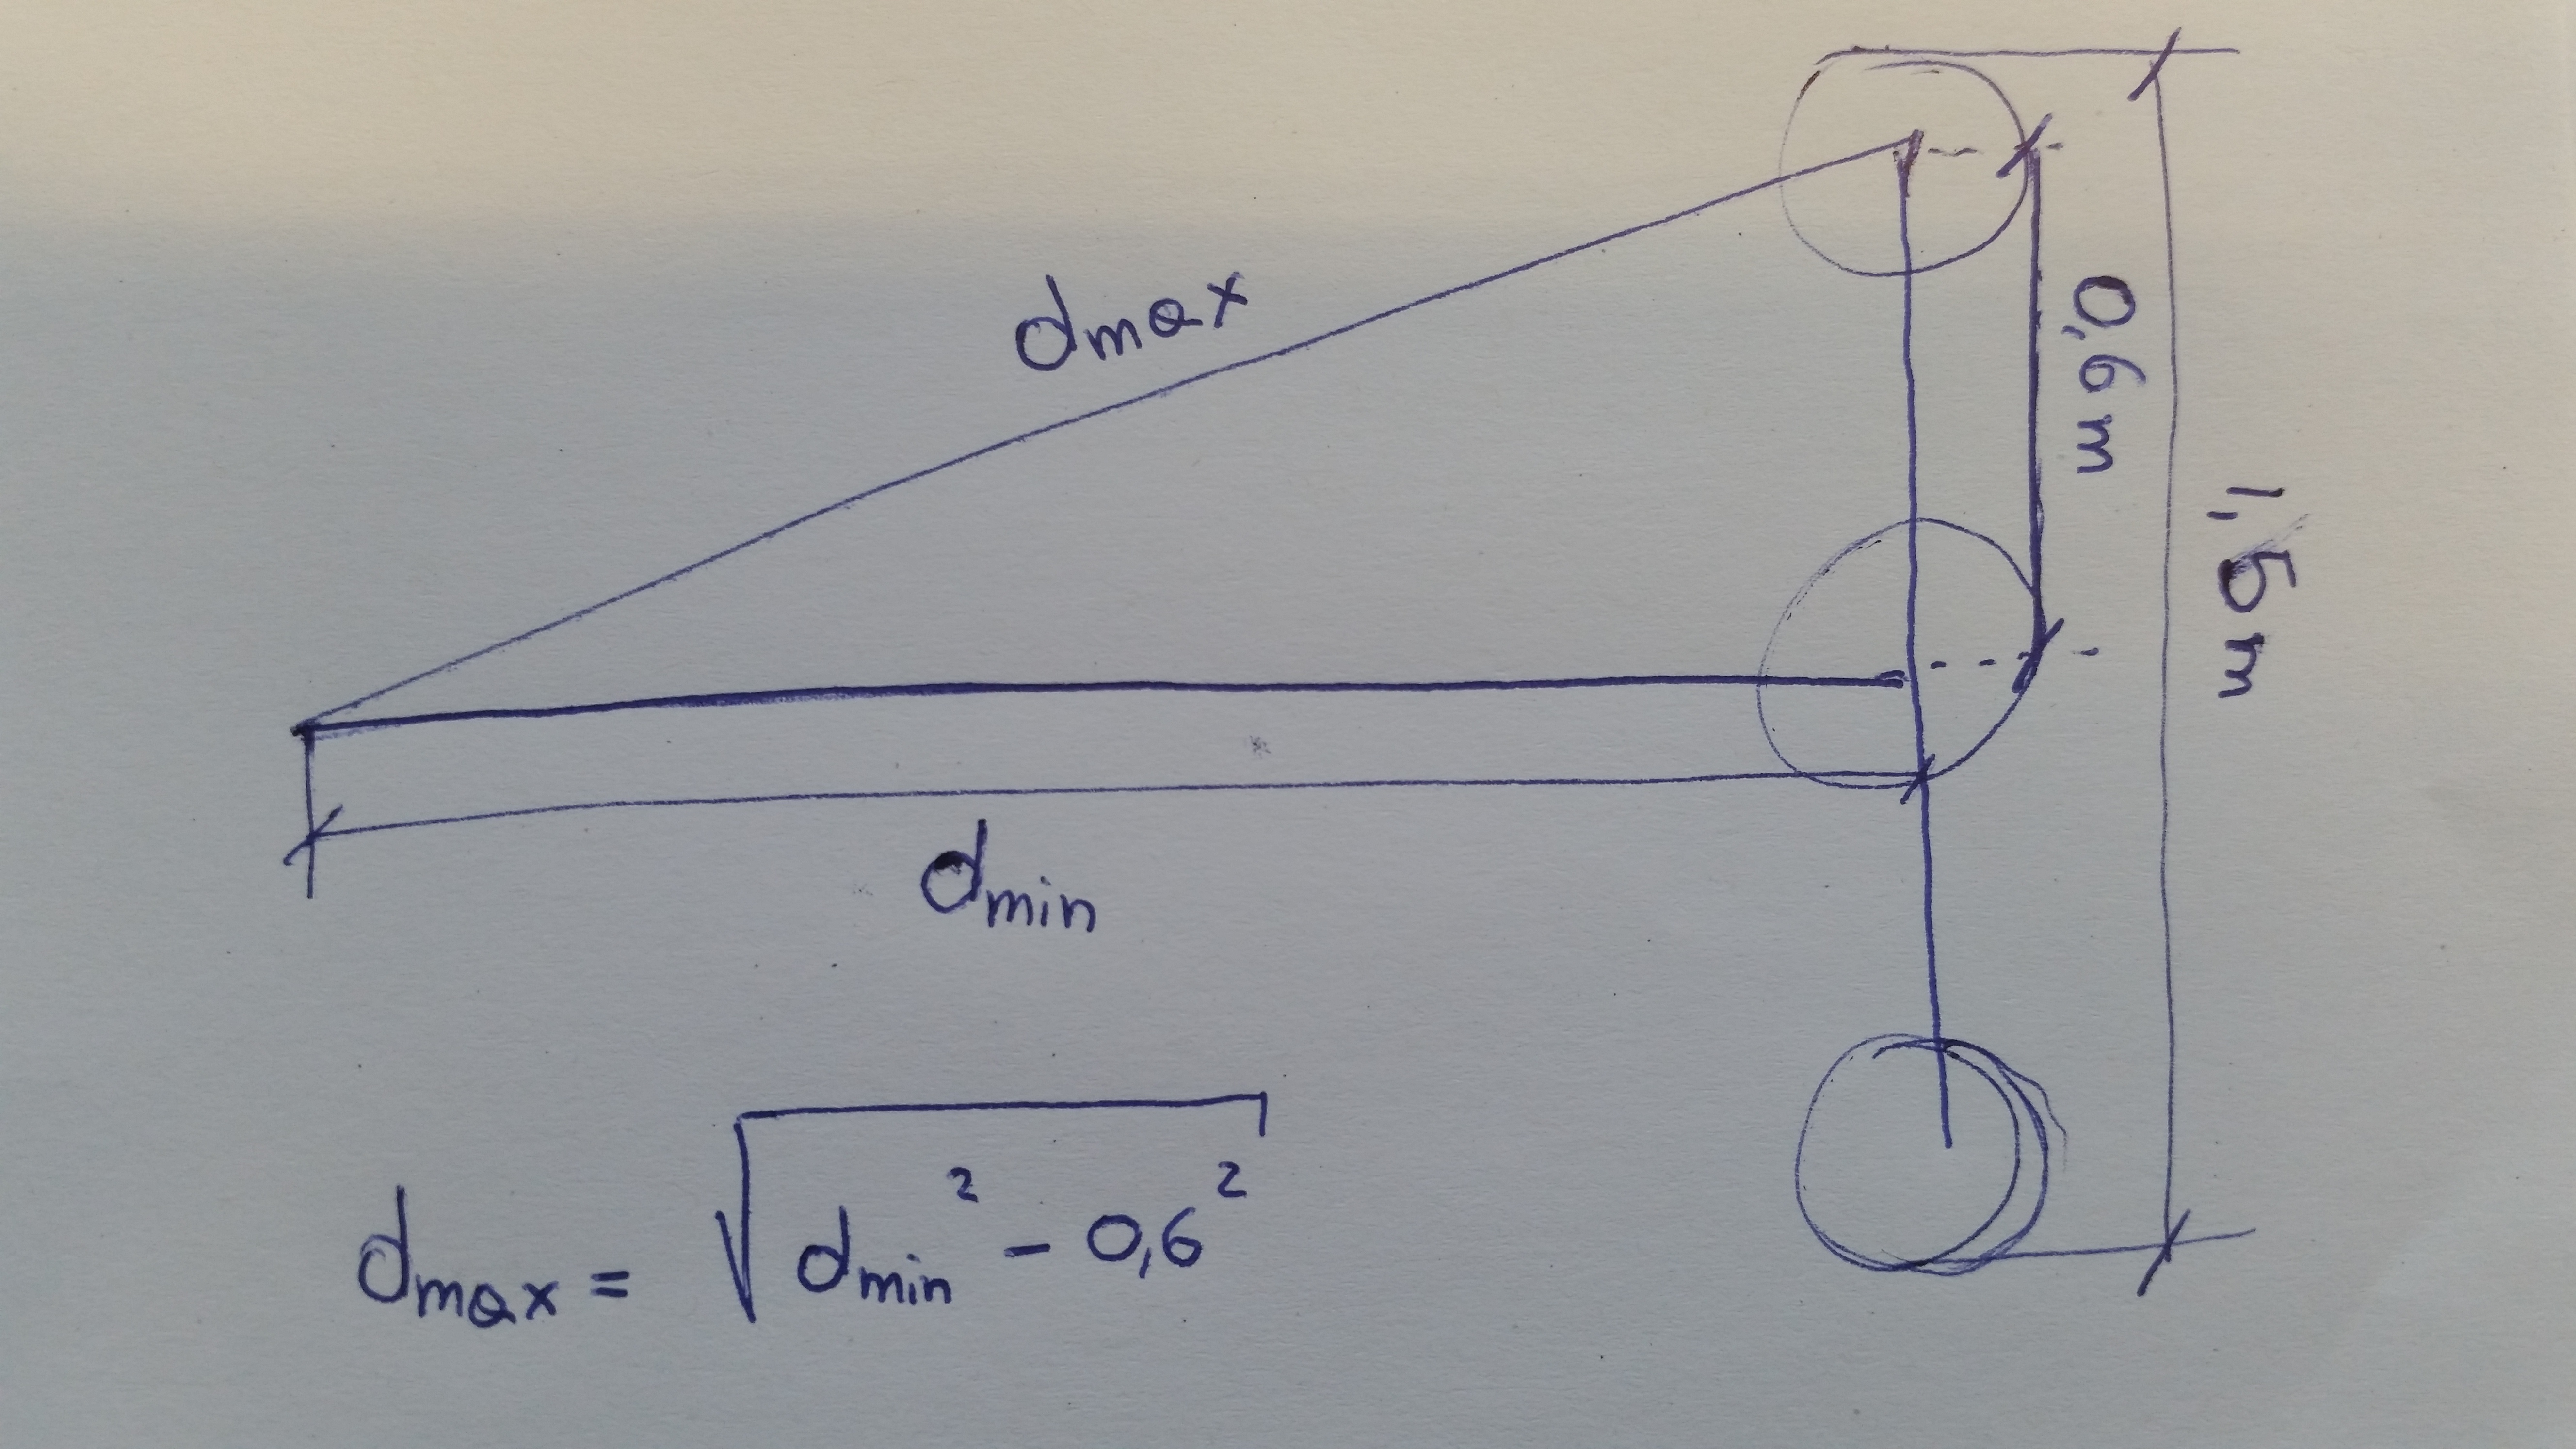
\includegraphics[width=1\textwidth]{../../fig/Skizze_Berechnung_2.jpg}
		\caption{Schräger Wurf von Oben}
	\end{subfigure}
	\caption{Berechnung schräger Wurf}
	\label{fig:berechnung_geschwindigkeiten}
\end{figure}

\begin{gather}
	v=\frac{\sqrt{g} \cdot d}{\sqrt{2} \cdot cos(\alpha) \cdot \sqrt{d \cdot tan(\alpha)+(h_0-h_1)}}\\
	\omega=\frac{v_{tan}}{r}\\
	f=\frac{\omega}{2\pi}\\
	rpm=60 \cdot f
\end{gather}

Die Berechnungen ergaben eine minimale Abwurfgeschwindigkeit von 4.18 m/s und eine Drehzahl von 532 U/min bei der kleinsten Wurfdistanz ($d_{min}$), 
Für die grösstmögliche Wurfdistanz ($d_{max}$) ergibt dies eine Geschwindigkeit von 4.29 m/s und eine Drehzahl von 546 U/min. 
Die Abweichung liegt bei rund 2.5\%.
Der Maximale Winkel zwischen der Mitte des Spielfeldes und der äussersten Position des Korbes $\alpha_{max}$ beträgt 19°.

Bei diesen Berechnungen sind Faktoren wie Reibung etc. nicht berücksichtigt. Aus diesem Grund sind die Resultate als Mindestanforderungen zu betrachten.

Um das erforderliche Drehmoment beim Drehrad zu bestimmen, wurde angenommen, dass der Ball eine Masse von 0.25 Kg (Gewicht des Balles und der Anpressdruck des Balles an das Drehrad) hat und das Drehrad wurde als Hebelarm angenommen. Mit diesen Annahmen wurde die Berechnung mit der folgenden Formel durchgeführt:

\begin{gather}
	M_{Drehmoment}=F*r
\end{gather}

Dies ergibt ein Drehmoment von 0.25 Nm. Auch in diesem Fall nehmen wir das als Mindestanforderung an.

Da eine Riemenscheibe benutzt wird, wird das Drehmoment am Motor mit einem Übersetzungsverhältnis von i=4 berechnet.

\begin{gather}
	M_{Antrieb}=\frac{M_{Abtrieb}}{i}
\end{gather}

Um auf der sichere Seite zu bleiben, rechnen wir mit einem Drehmoment von 0.5 Nm am Rad und einem Moment von 0.125 Nm am Motor.

Für die Berechnungen der Daten vom Schrittmotor, der für die Drehung zuständig ist, haben wir die Maschine auf 2 Teile reduziert: Platte und Aufbau.
Die Platte ist ein Zylinder mit $r=0.25$m und $h=0.005$m, da die Durchschnittliche Dichte der Holz ist $750 Kg/m^2$, ergibt sich eine Masse von ca. 0.75 Kg.
Der Aufbau ist ein Quader mit $l=0.5$m, $b=0.01$m und wir schätzen eine Masse von 4 Kg.

Mit diesen Daten wurde das mögliche Trägheitsmoment berechnen.

\begin{gather}
	I_{Platte}=\frac{1}{2}*m*r^2 \\
	I_{Aufbau}=\frac{1}{12}*m*(l^2+b^2)
\end{gather}

Das gesamte Trägheitsmoment ist somit $I=0.18 Kg*m^2$.

Die Maschine, wenn sie in der Mitte des Spielfeldes positioniert wird, muss sich maximal um 19$^\circ$ nach links und rechst drehen können. Wenn für diese Bewegung eine Zeit von 1 Sekunde festlegt wird, kann man die Winkelbeschleunigung berechnen.

\begin{gather}
	\theta(t)=\theta_0+\omega_0*t+\frac{1}{2}*\alpha*t^2
\end{gather}

Man erhält so eine Winkelbeschleunigung $\alpha$ von $0.66\frac{rad}{s^2}$.
Mit dem Trägheitsmoment und der Winkelbeschleunigung kann das Drehmoment mit folgender Formel berechnet werden: $M=\alpha*I$. Dies ergibt ein Drehmoment von 0.12 Nm.

Die Kraft welche benötigt wird, um die Bälle dem Drehrad zuzuführen, wurde mit folgenden Annahmen berechnet. Alle 5 Bälle werden zusammen vertikal angehoben. Die 5 Bälle haben eine Masse von $60*5=300$g. Diese 300g ergeben eine Kraft von $F_g=0.3*9.81\approx3 N$. Um mit dieser Kraft das Drehmoment zu berechnen, wurde mit einer Scheibe welche grösser ist als der Radius der Bälle ($r=3.7cm$) gerechnet. Um mit etwas Sicherheit weiterzufahren, wurde mit einem Radius von 5 cm fortgefahren. Das benötigte Drehmoment beträgt somit $M=F*r$, 0.15 Nm.
In der Tabelle \ref{fig:drehmoment} sind alle Resultate zusammengefasst.

\begin{figure}[h!]
	\center
	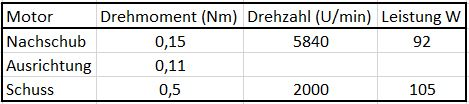
\includegraphics[width=0.5\textwidth]{../../fig/Tabelle_Drehmomente.jpg}
	\caption{Drehmoment, Drehzahl und Leistung der Motoren}
	\label{fig:drehmoment}
\end{figure} 
\newpage

\subsubsection{Sichtfeld der Kamera}
\label{subsub:sichtfeld-der-kamera}
Damit sichergestellt werden kann dass die Kamera das gesamte Spielfeld fotografieren kann, wird in diesem Abschnitt das Sichtfeld der Kamera berechnet. Auf der Website von \citeauthor{raspberry-pi-camera} \citeyear{raspberry-pi-camera} wurden diverse Tests mit dem Raspberry Pi Camera Modul (siehe Abschnitt \ref{subsub:kamera}) durchgeführt. Diese haben ergeben dass die Kamera ein horizontales Sichtfeld von $53^\circ$ und ein vertikales Sichtfeld von $40^\circ$ hat. Wie man der Abbildung \ref{fig:berechnung_sichtfeld} entnehmen kann ergibt das bei einer Distanz von zwei Meter eine Aufnahmefläche von 2×1.3 Meter.

\begin{figure}[h!]
\centering
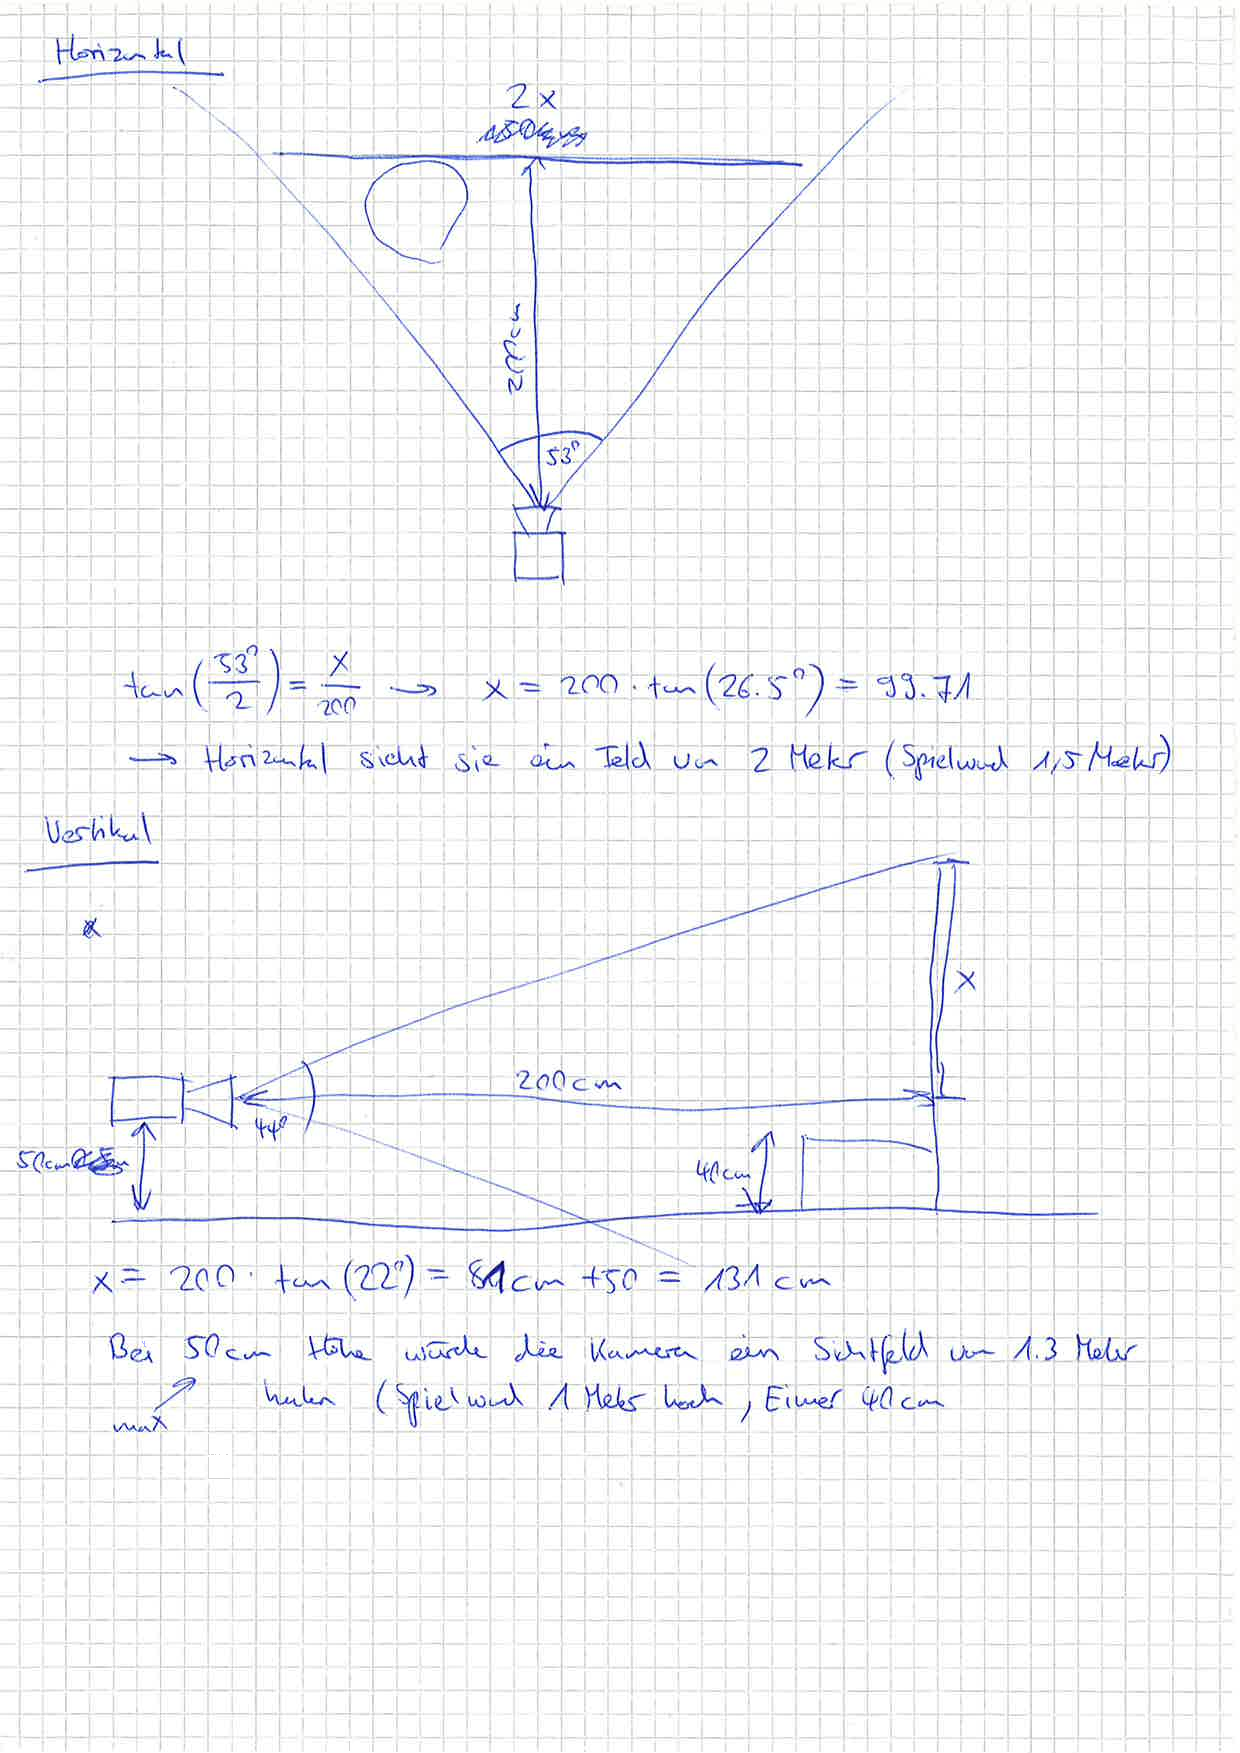
\includegraphics[width=0.6\linewidth]{../../fig/berechnung_sichtfeld.pdf}
\caption{Berechnung des Sichtfeldes der Kamera}
\label{fig:berechnung_sichtfeld}
\end{figure}


\subsubsection{Weitere Berechnungen}
Detailliertere Berechnungen sind im Anhang zu finden (siehe \ref{anhang-Berechnungen})